\documentclass[10pt]{beamer}
% Class options include: notes, notesonly, handout, trans,
%                        hidesubsections, shadesubsections,
%                        inrow, blue, red, grey, brown

% Theme for beamer presentation.
\usepackage{beamerthemesplit} 
%\usepackage{times}
\usepackage{anysize}
\usepackage{fancyhdr}
\usepackage{graphicx}
\usepackage{pdfpages}
\usepackage{amsmath}
\usepackage{amssymb}
% Other themes include: beamerthemebars, beamerthemelined, 
%                       beamerthemetree, beamerthemetreebars  

\title{Jafar --- Intelligent Othello Agent}    % Enter your title between curly braces
\author{Joshua Nelson, Tim Cosgrove, Andrew Haigh}                 % Enter your name between curly braces
\institute{COMP3130 Research Project}      % Enter your institute name between curly braces
\date{\today}                    % Enter the date or \today between curly braces

\usetheme{PaloAlto}
\usecolortheme{crane}

\newcommand{\bcen}{\begin{center}}
\newcommand{\ecen}{\end{center}}

\begin{document}

% Creates title page of slide show using above information
\begin{frame}
  \titlepage
\end{frame}
\note{} % Add notes to yourself that will be displayed when
        % typeset with the notes or notesonly class options

\section[Outline]{}

% Creates table of contents slide incorporating
% all \section and \subsection commands
\begin{frame}
  
  \begin{columns}[c]
  \column{2in}
  \tableofcontents
  \column{2in}
  \framebox{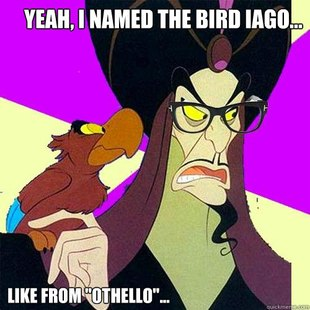
\includegraphics[height=4cm]{hipsterjafar}}
  \end{columns}
\end{frame}


\section{Problem Overview}

\begin{frame}
  \frametitle{Problem Overview}   % Insert frame title between curly braces
  \begin{columns}[c]
  \column{2in}  % slides are 3in high by 5in wide
  \begin{itemize}
  \item<1-> The Game --- 10x10 Modified Othello
  \item<2-> The Problem --- Intelligent AI player
  \item<3-> Solution basis
  \end{itemize}
  \column{2in}
  \framebox{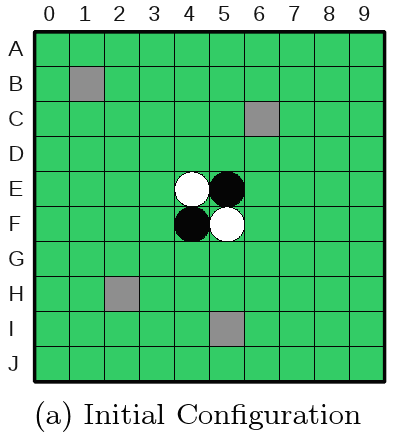
\includegraphics[height=5cm]{initconfig}}
  \end{columns}
\end{frame}

\section{Solution Structure}

\begin{frame}
  \frametitle{Solution Structure}   % Insert frame title between curly braces
  \begin{itemize}
  \item<1-> The MetaPlayer class --- Utilises knowledge of the game state and 
        creates instances of other players accordingly
  \item<2-> NegamaxPlayer (varying depth argument)
  \begin{itemize}
    \item<2-> The 'main' AI player; performs a pruned Negamax search (simplification of Minimax)
    \item<2-> Searches to a depth specified by the MetaPlayer; where it then
    evaluates the quality of the leaf states
  \end{itemize}
  \item<3-> Other Player interfaces:
  \begin{itemize}
    \item<3-> OpeningPlayer
    \item<3-> GreedyPlayer
    \item<3-> HumanPlayer
  \end{itemize}
  \end{itemize}
\end{frame}

\section{Static Evaluation}

\begin{frame}
  \frametitle{Static Evaluation}   % Insert frame title between curly braces
  \begin{itemize}
  \item<1-> The FeatureSet class --- Maintains a list of \emph{features}; functions
  which evaluate a game state based on some criteria of strength
  \item<2-> LegalMoves Feature
  \begin{itemize}
    \item<2-> Also known as 'mobility'; the number of moves available to the agent
    \item<2-> Having only a few moves available is very limiting
    \item<2-> Useful through all stages of the game
  \end{itemize}
  \end{itemize}
\end{frame}

\begin{frame}
  \frametitle{More Features}   % Insert frame title between curly braces
  \begin{itemize}
  \item<1-> BlockedAdjacent, CornerPieces, SidePieces
  \begin{itemize}
    \item<2-> Count of how many pieces we have next to blocked squares, corners and edges
    \item<2-> Useful as these pieces are harder to capture; easier to 'lock'
  \end{itemize}
  \item<3-> Visibility
  \item<3-> StoneCount
  \end{itemize}
\end{frame}

\section{TD-$\lambda$}
\subsection{Algorithm description}
    \begin{frame}
      \frametitle{TD-$\lambda$}
      \begin{itemize}
        \item<1-> Remaining challenge: decide how important each feature is\\ (the feature 'weights')
        \item<2-> Solution - use the TD $\lambda$ (Temporal Difference) formula to calculate the new weights
        \item<2-> $\displaystyle w := w + \alpha \sum_{T=1}^{N-1} \tilde{J}(x_t,w) *( \sum _{j=t} ^{N-1} \lambda ^{j-t} d_t )$ 
      \end{itemize}
    \end{frame}
    
    \begin{frame}
      \frametitle{The J Function}
      \begin{center} $\displaystyle w := w + \alpha \sum_{T=1}^{N-1} \Delta \tilde{J}(x_t,w)$  \textcolor{gray}{$ * ( \sum _{j=t} ^{N-1} \lambda ^{j-t} d_t )$} \end{center}
      \begin{itemize}
        \item<1-> The J function returns a probability of winning, given a set of weights and a board.
        \item<1-> The perfect J function would always return 0 or 1 precisely.
        \item<1-> We are trying to learn a good approximation to the J function
      \end{itemize}
    \end{frame}
    
    \begin{frame}
      \frametitle{TD: Temporal difference}
      \begin{center} \textcolor{gray}{$\displaystyle w := w + \alpha \sum_{T=1}^{N-1} \Delta \tilde{J}(x_t,w) *$}  $( \sum _{j=t} ^{N-1} \lambda ^{j-t} d_t )$ \end{center}
      \begin{itemize}
        \item<1-> $d_t$ is the \emph{Temporal Difference} between successive game states.
        \item<1-> The key observation is that for an ideal J function this would always be zero.
        \item<1-> $\Delta \tilde{J}(x_t,w)$ corrects each weight according to whether it was pointing us in the right direction.
      \end{itemize}
    \end{frame}

\subsection{Results}



\begin{frame}
  \frametitle{Initial J function}
  \framesubtitle{Lost game}
  \begin{center} 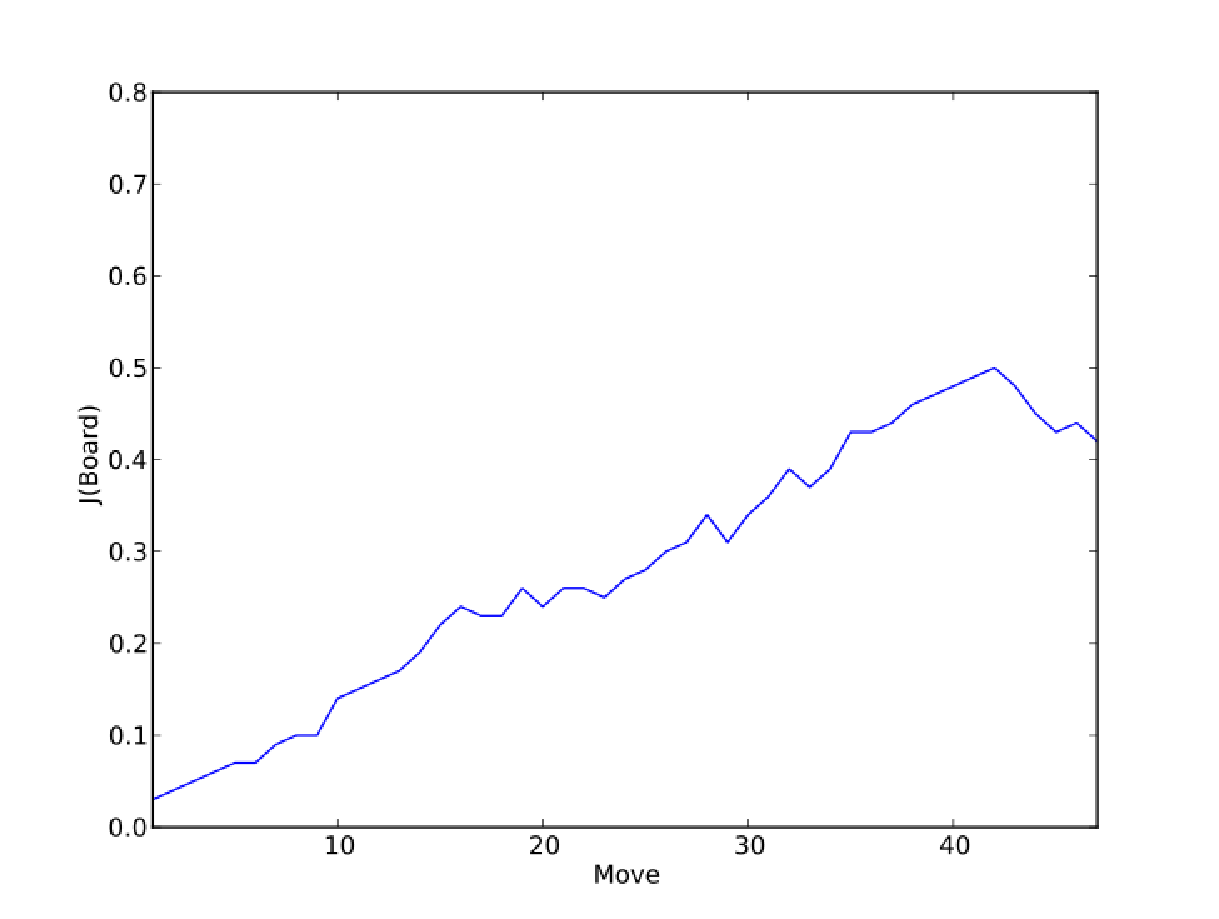
\includegraphics[height=6cm]{Graphs/J_1iteration_lost.pdf} \end{center}
\end{frame}

\begin{frame}
  \frametitle{J function after 6000 iterations}
  \framesubtitle{Lost game}
  \begin{center} 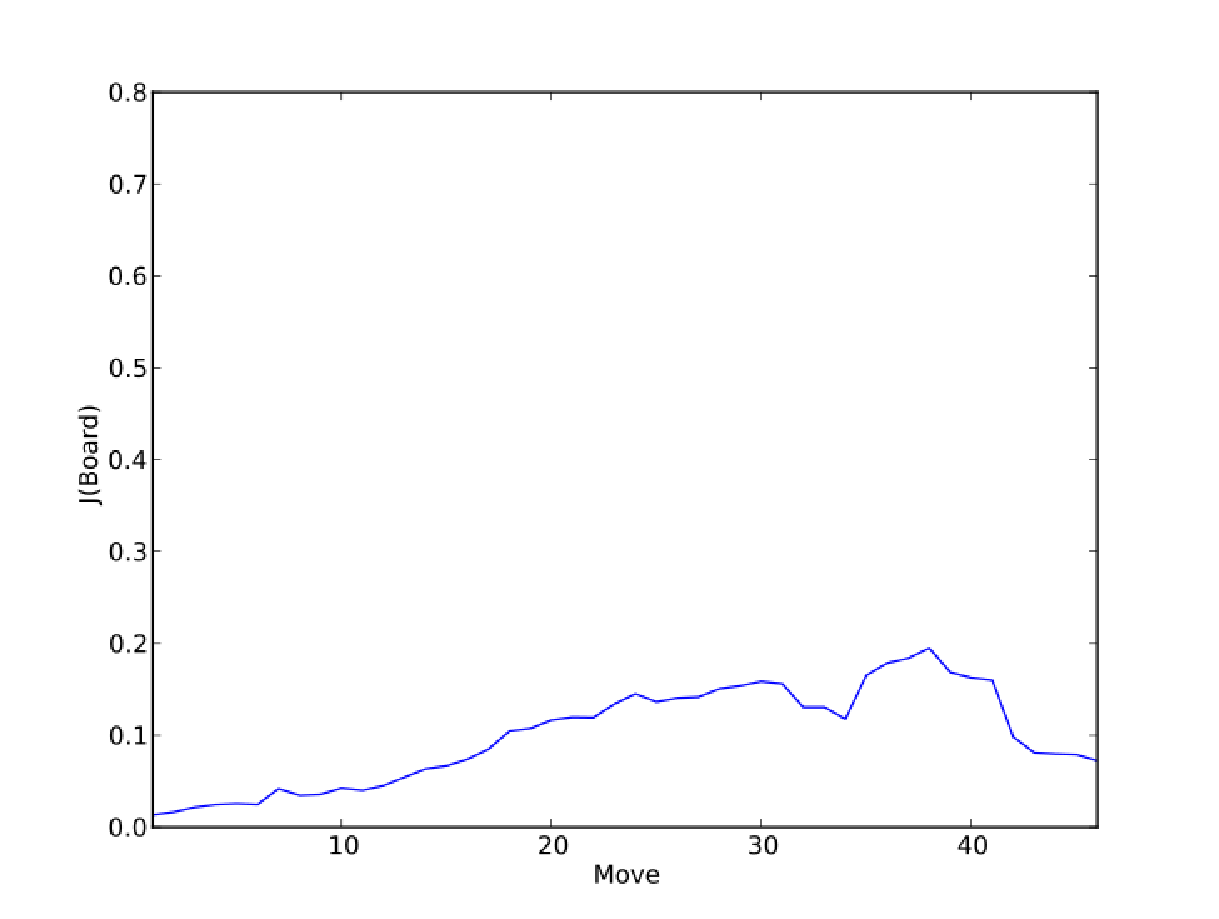
\includegraphics[height=6cm]{Graphs/J_6000iterations_lost.pdf} \end{center}
\end{frame}

\begin{frame}
  \frametitle{J function after 6000 iterations}
  \framesubtitle{Won game}
  \begin{center} 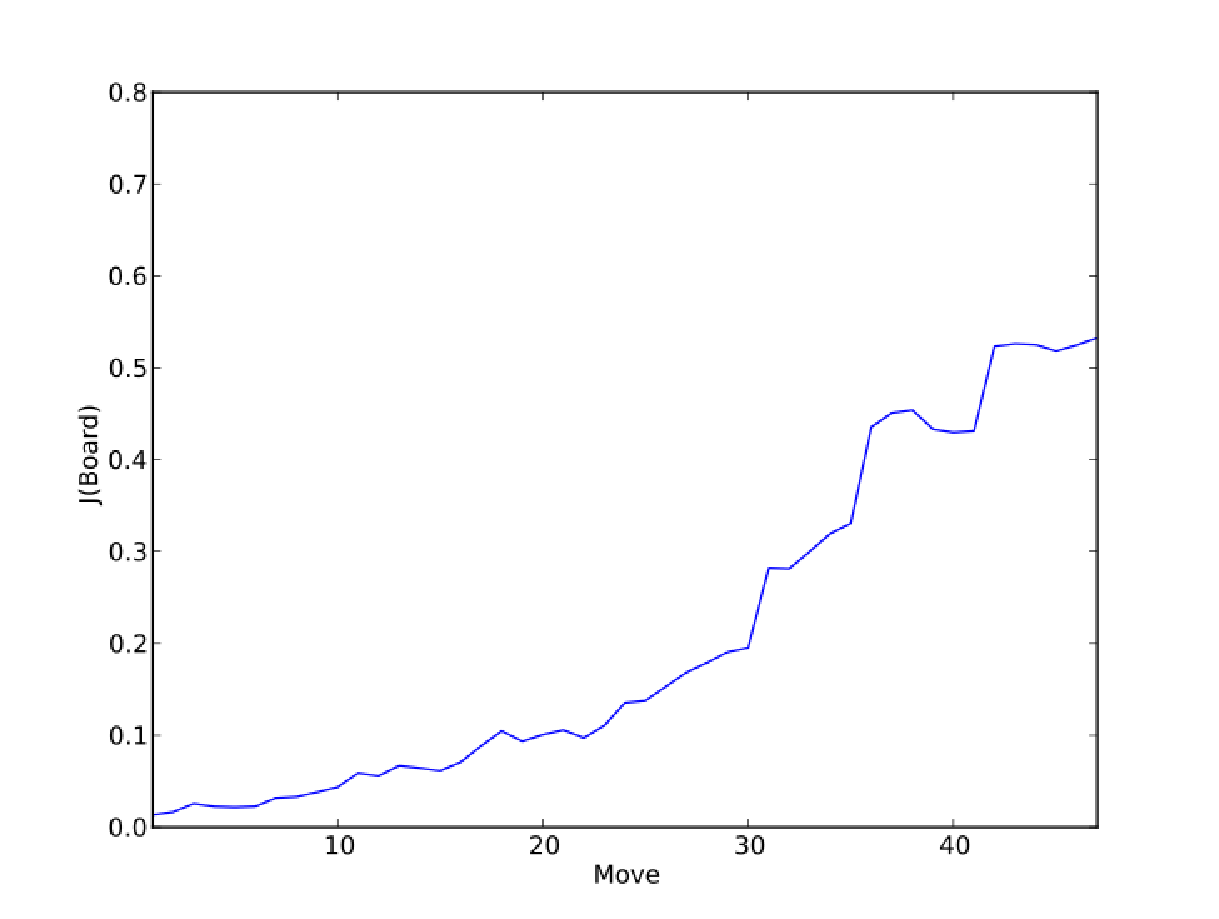
\includegraphics[height=6cm]{Graphs/J_6000iterations_win.pdf} \end{center}
\end{frame}

\begin{frame}
  \frametitle{The first 1000 learning iterations}
  \begin{center} 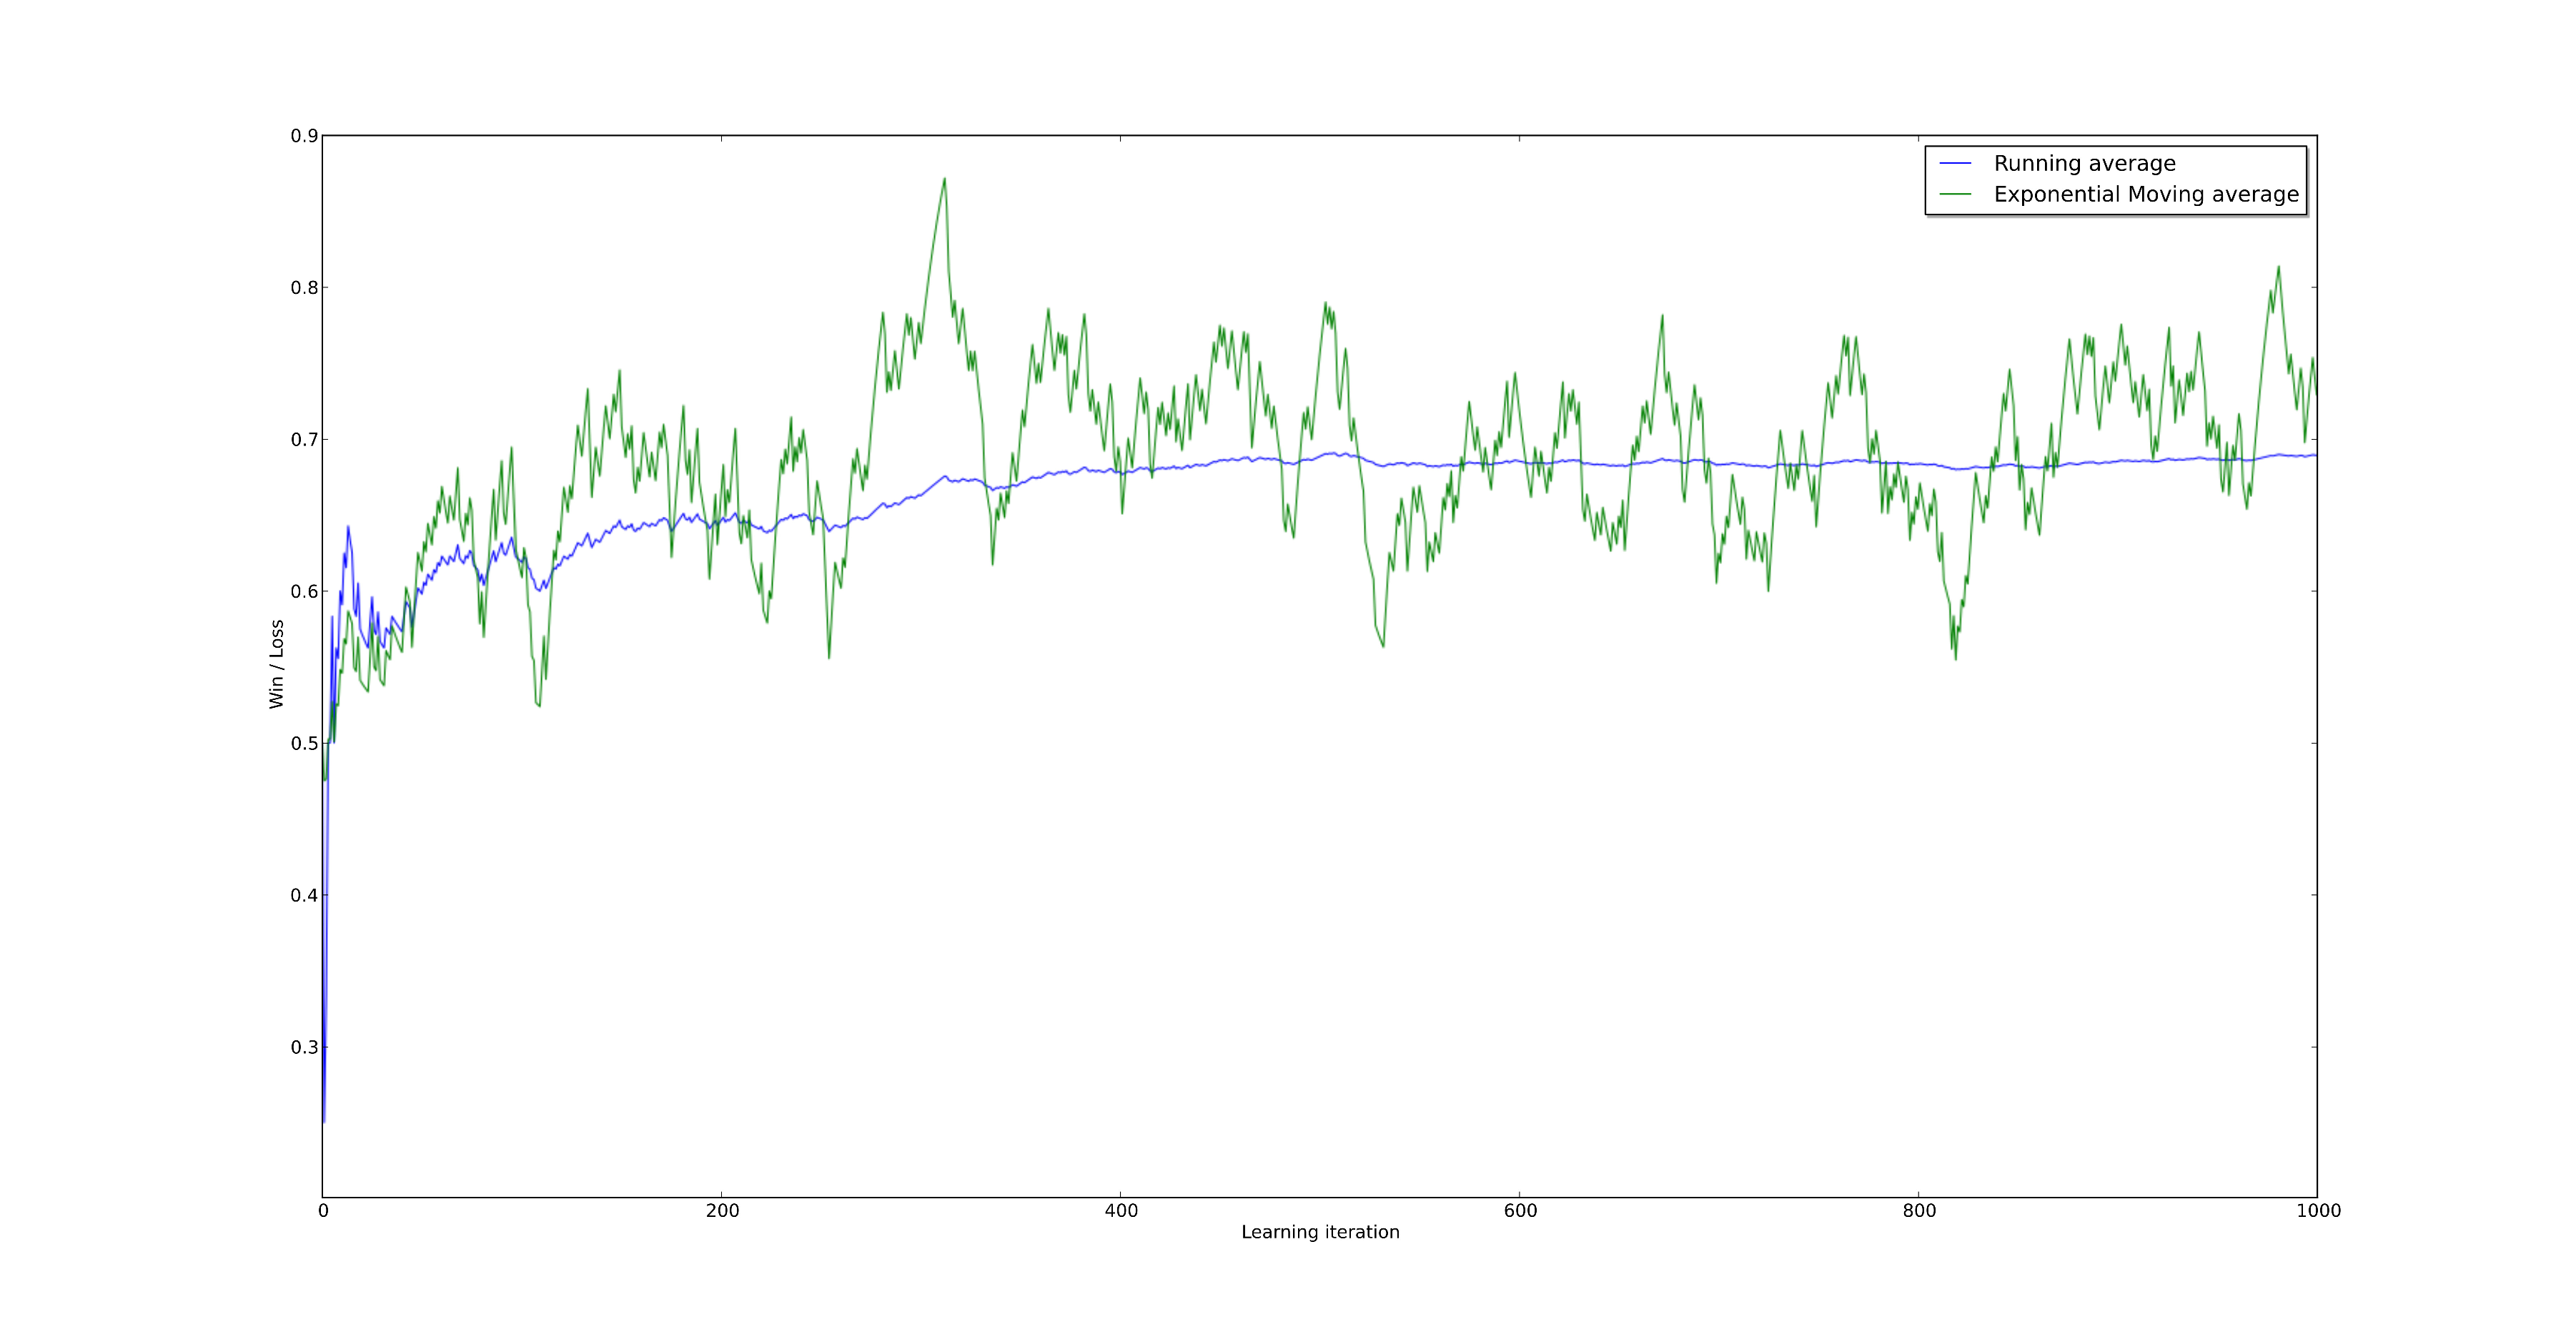
\includegraphics[trim= 6cm 2cm 2cm 2cm, clip, height=5.6cm]{Graphs/Learning_2ply_First1000.pdf} \end{center}
\end{frame}

\begin{frame}
  \frametitle{The first 5000 learning iterations}
  \begin{center} 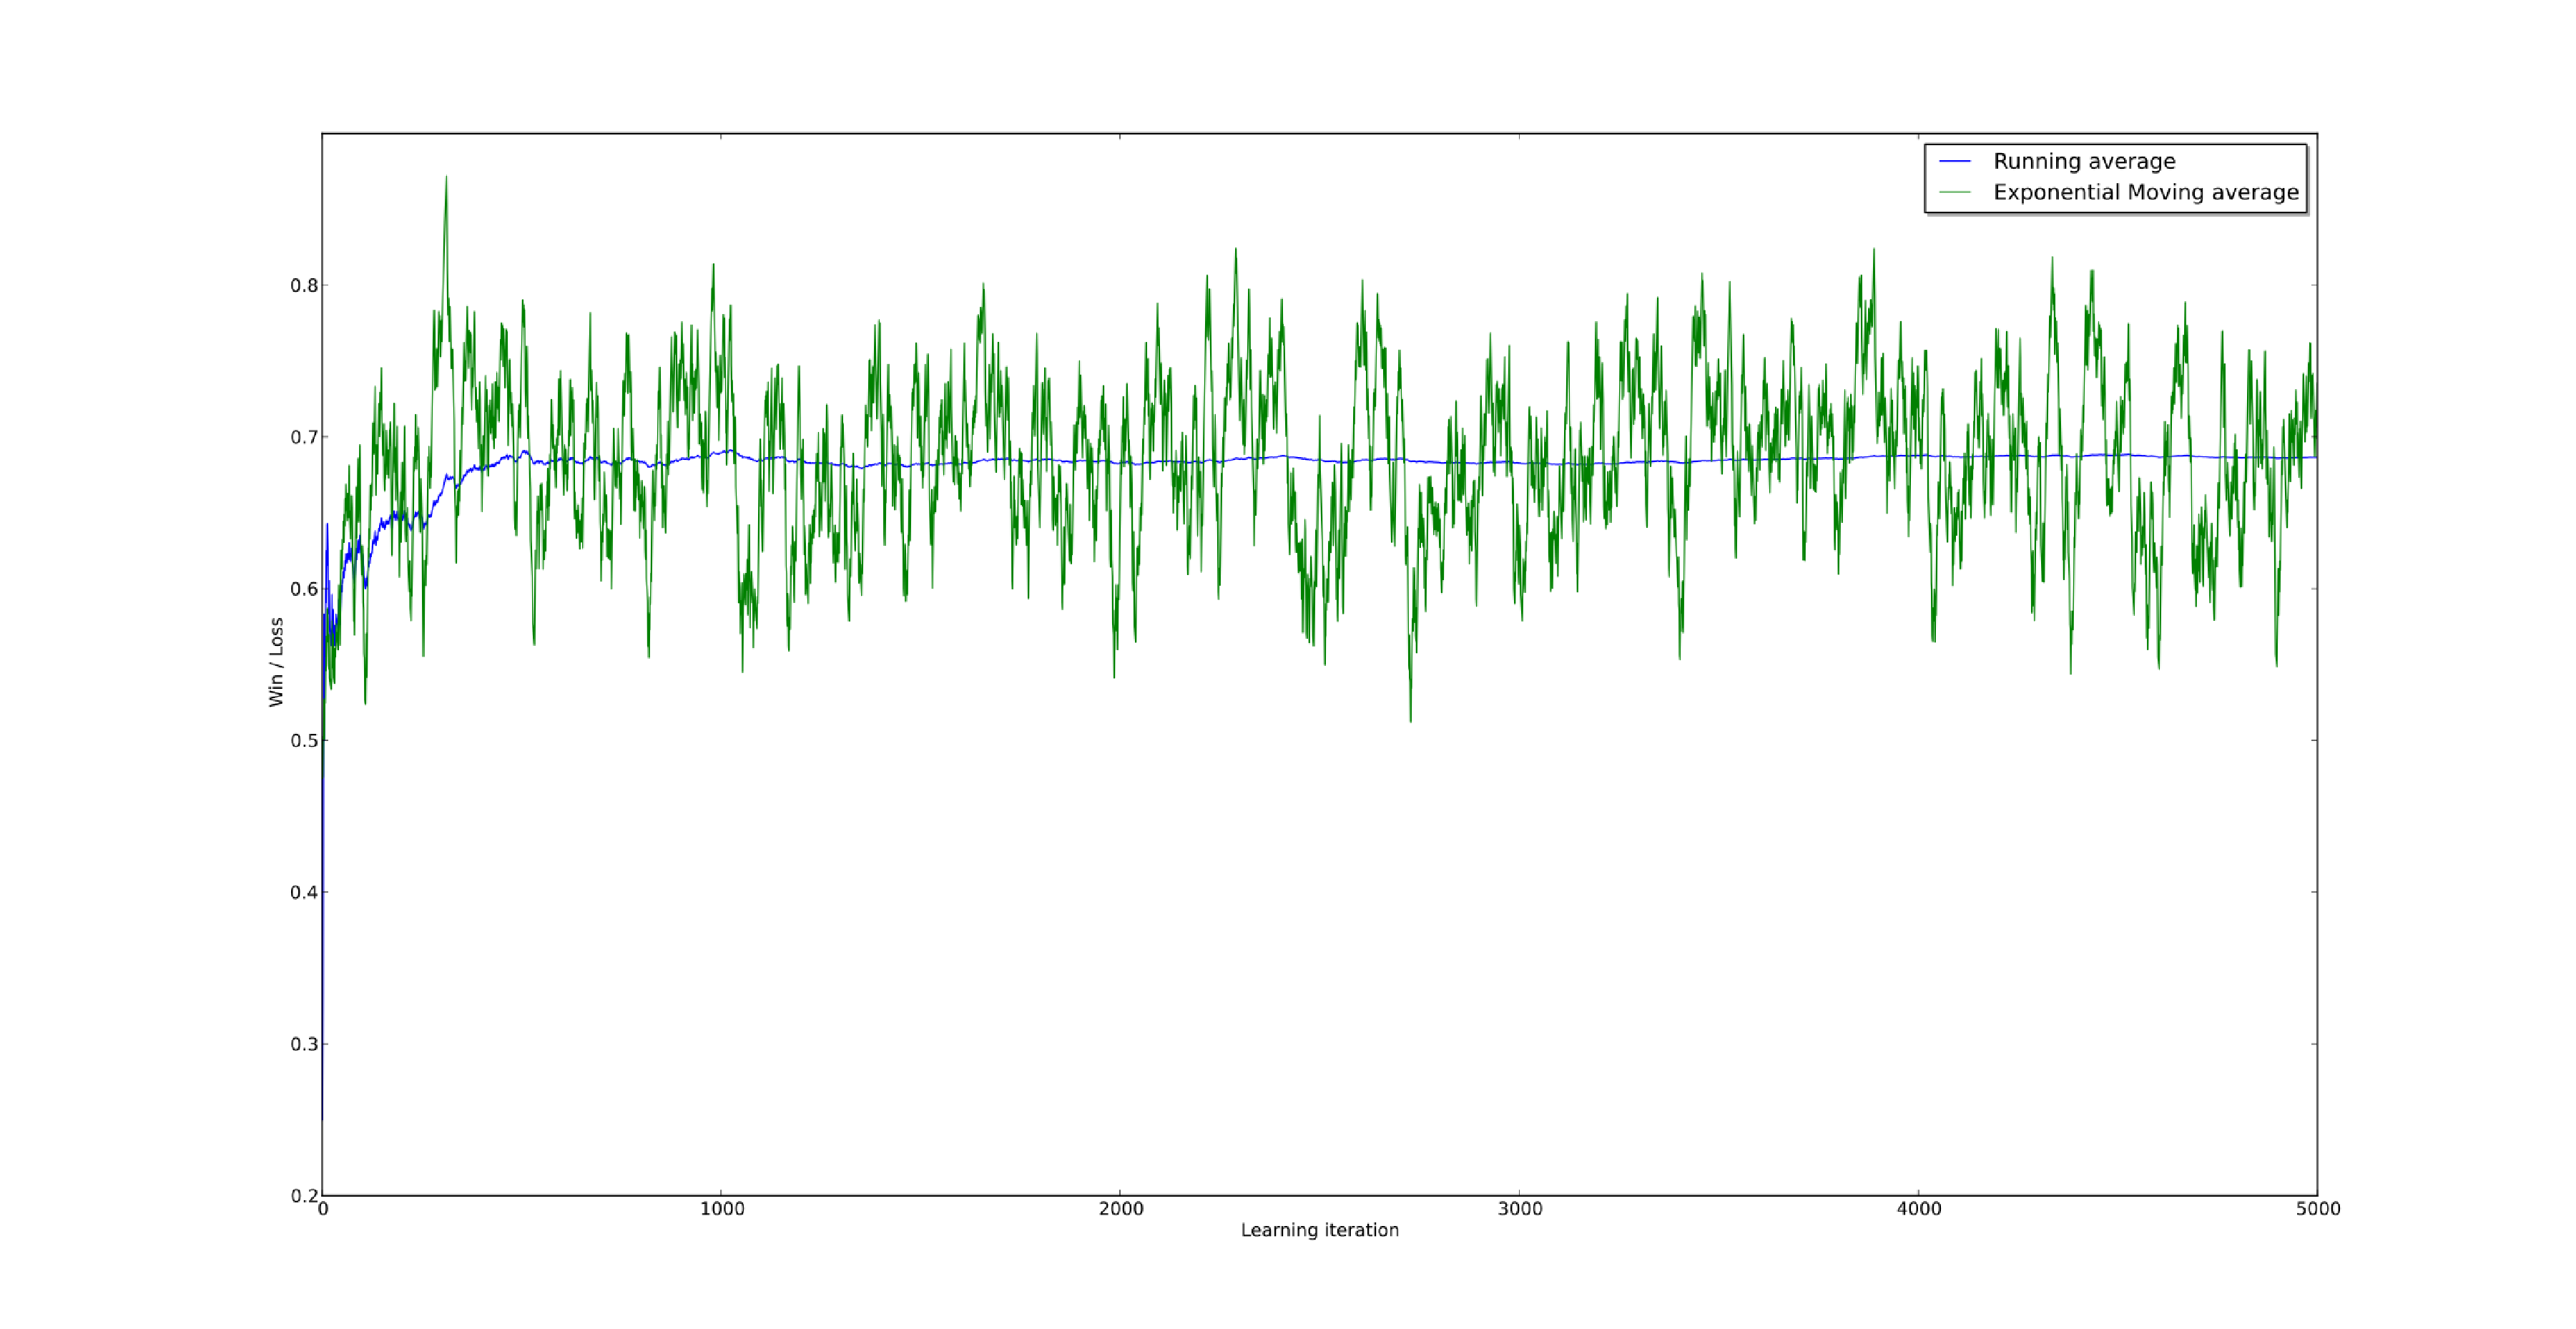
\includegraphics[trim= 6cm 2cm 2cm 2cm, clip, height=5.6cm]{Graphs/Learning_2ply_First5000_exp.pdf} \end{center}
\end{frame}

\begin{frame}
  \frametitle{Self play - learnt weights}
  \begin{center} 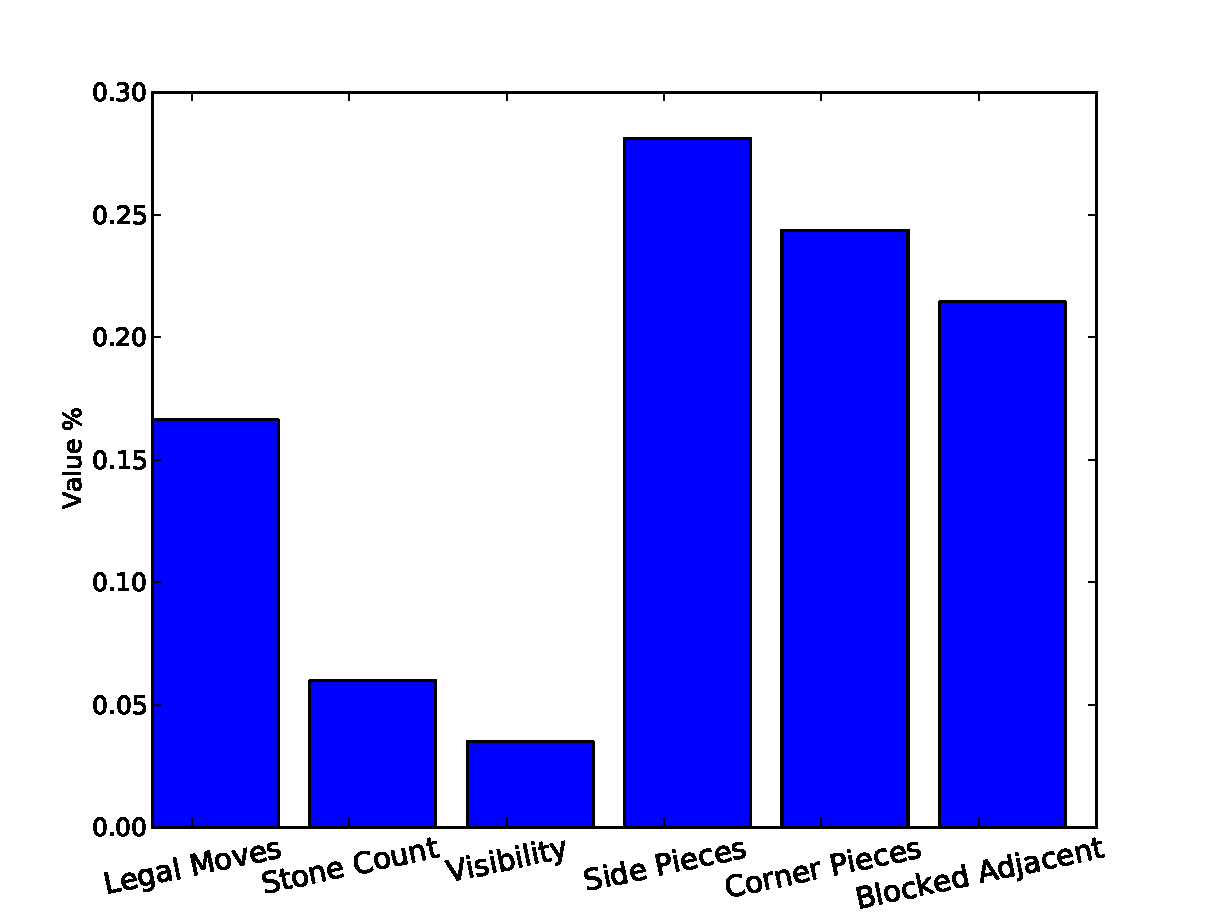
\includegraphics[height=6cm]{Graphs/SelfPlay_Weights.pdf}  \end{center} 
\end{frame}

\begin{frame}
  \frametitle{Self play - learnt weights}
  \framesubtitle{White - Black}
  \begin{center} 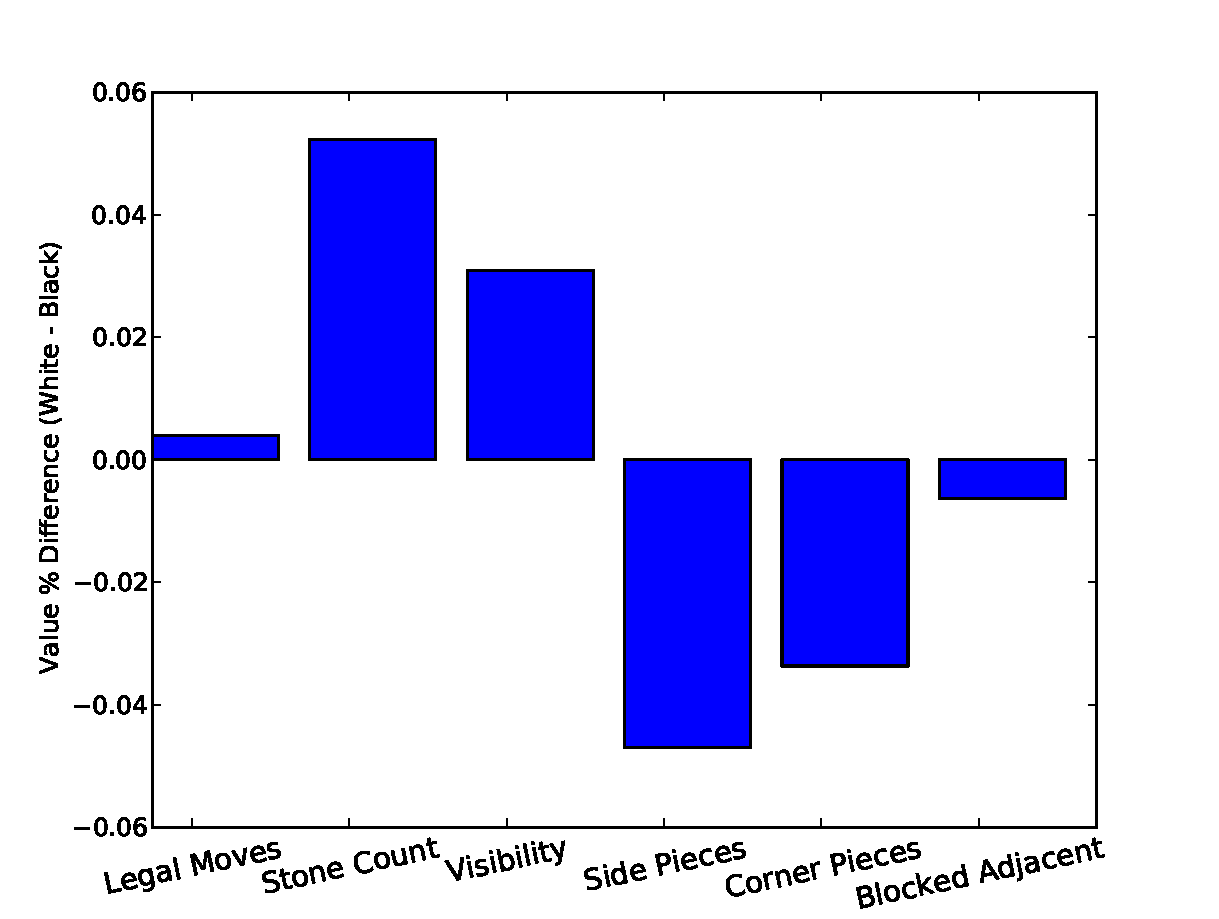
\includegraphics[height=6cm]{Graphs/SelfPlay_Weights_WhiteBlackDiff.pdf}  \end{center} 
\end{frame}

\begin{frame}
  \frametitle{Feature weight space visualisation}
  \begin{center} 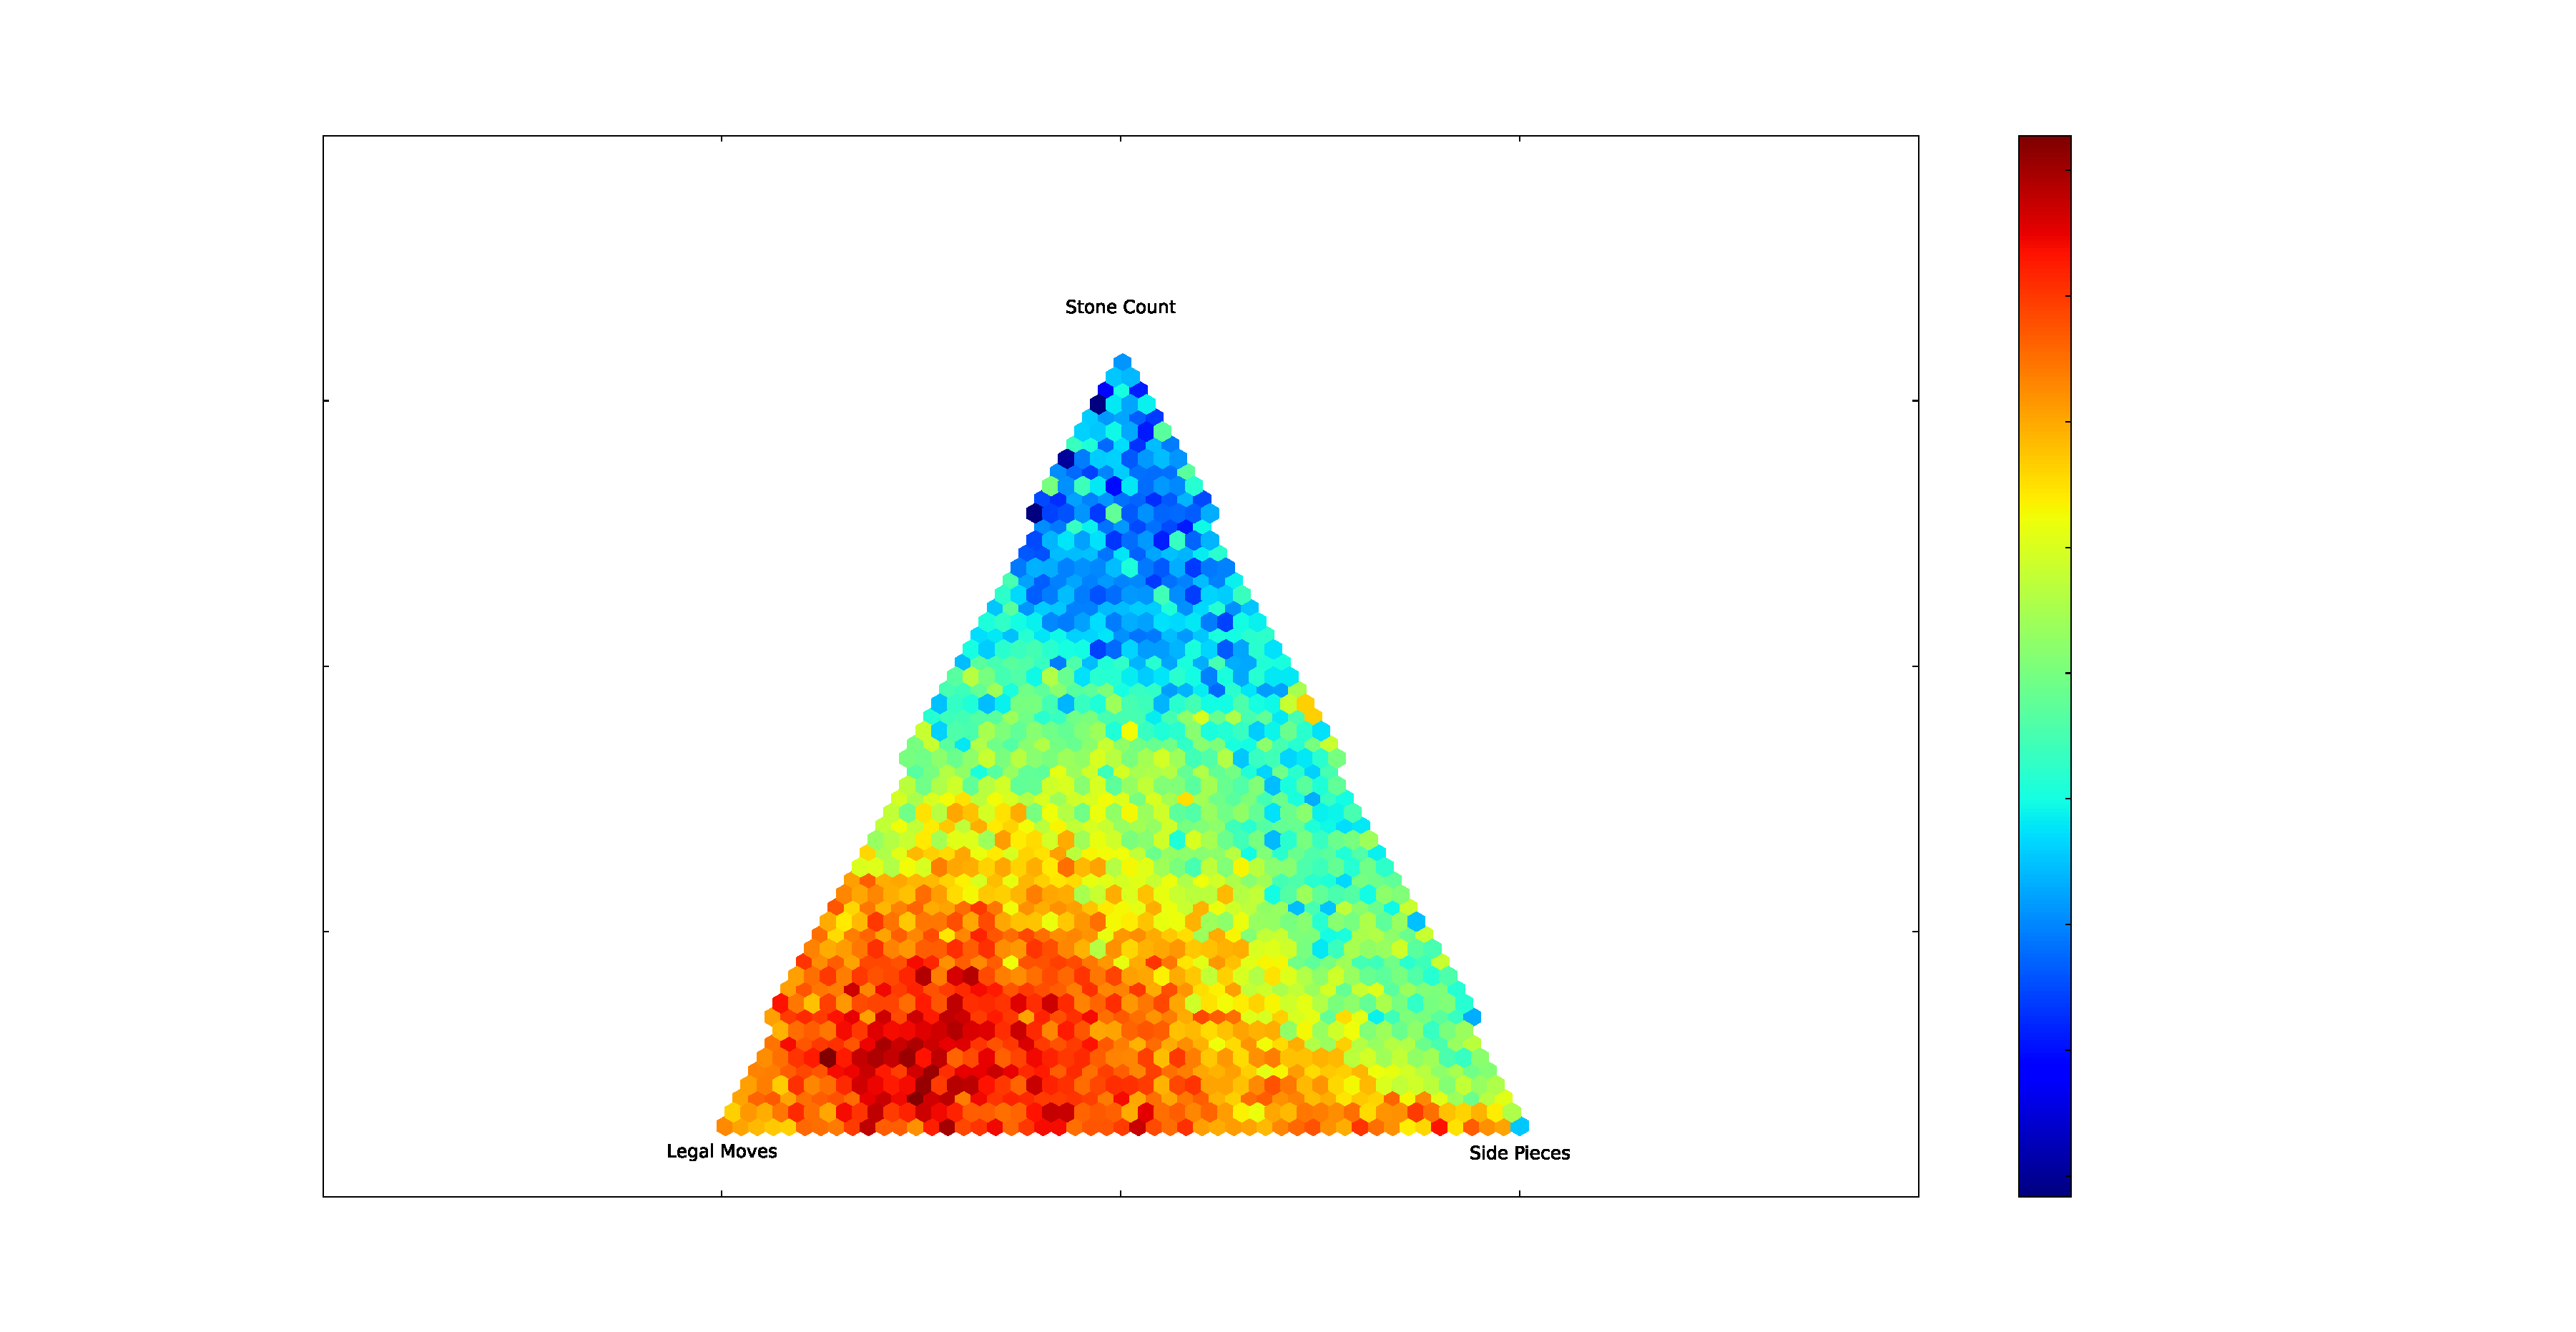
\includegraphics[trim= 12cm 4cm 23cm 7cm, clip, height=7cm]{Graphs/LegalMoves_Count_SidePieces_Triangle.pdf}  \end{center}
\end{frame}

\begin{frame}
  \frametitle{Feature weight space visualisation}
  \begin{center} 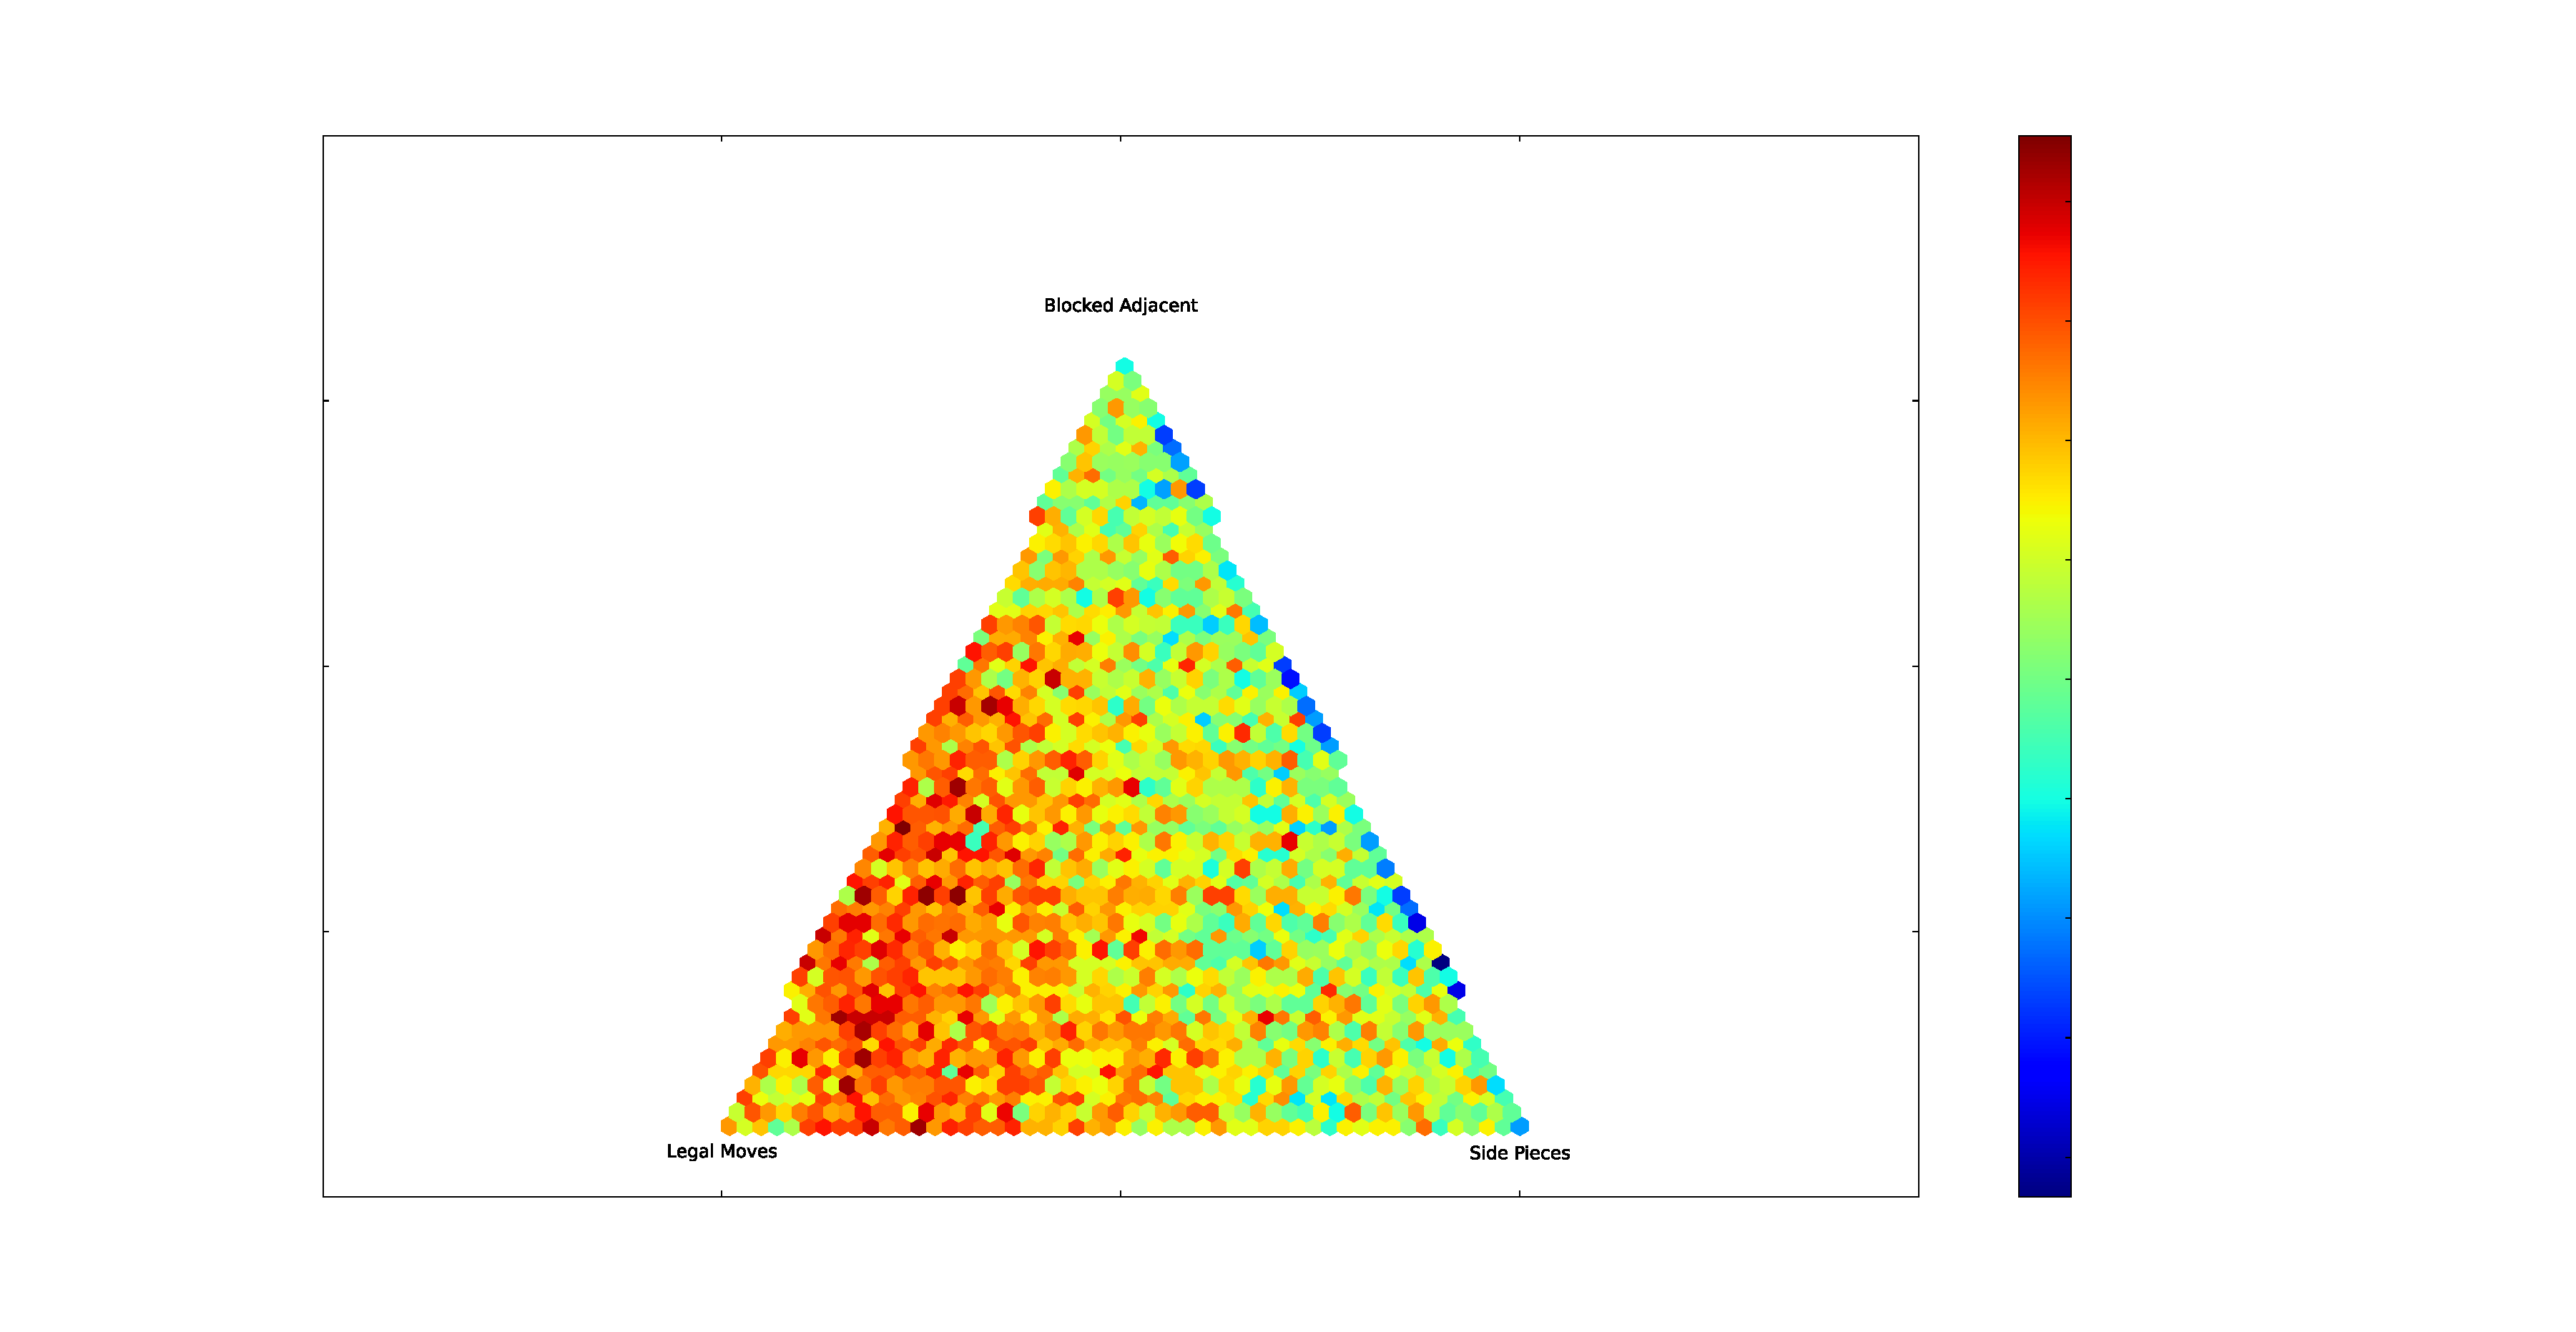
\includegraphics[trim= 12cm 4cm 23cm 7cm, clip, height=7cm]{Graphs/LegalMoves_BlockedAdjacent_SidePieces_Triangle.pdf}  \end{center} 
\end{frame}

\section{The EloArena}

\begin{frame}
  \frametitle{The Elo Rankings Arena}
  \begin{itemize}
  \item<1-> Custom made genetic algorithm
  \item<1-> Pits a group of randomly generated agents against each other for Elo style ranking points
  \item<1-> Creates new agents from those who perform best
  \item<2-> Used more as a demonstration of the learning process
  \item<2-> Interesting to see it come to the same conclusions as TD-$\lambda$
  \end{itemize}
\end{frame}

\section{Future Improvements}

\begin{frame}
  \frametitle{Future Improvements}
  \begin{itemize}
  \item<1-> More attention to blocked squares
  \item<2-> Negamax optimisations (better transposition tables, prob-cuts)
  \item<3-> Better use of pre-computed data (such as the Opening Book)
  \item<4-> More board features (locked squares, open squares, etc.)
  \item<5-> Generic features (features learnt by the agent)
  \item<6-> More exploration in learning - randomise the initial board and play from that to explore more options
  \end{itemize}
\end{frame}

\section{Design Methodology}

\begin{frame}
\frametitle{Design Methodology}
  \begin{itemize}
  \item<1-> C with a python interface
      \begin{itemize}
        \item<1-> Used this for tic-tac-toe warm up problem, decided against due to development overhead 
      \end{itemize}
  \item<2-> Java
      \begin{itemize}
        \item<2->  Sacrifice low level speed improvements for high level language features and built in data structures.
      \end{itemize}
  \end{itemize}
\end{frame}

\begin{frame}
\frametitle{Design Methodology}
  \bcen
  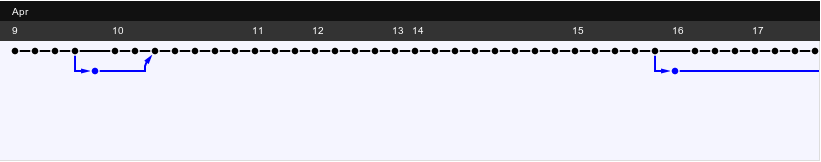
\includegraphics[height=1.3cm,width=7cm]{line1}\\
  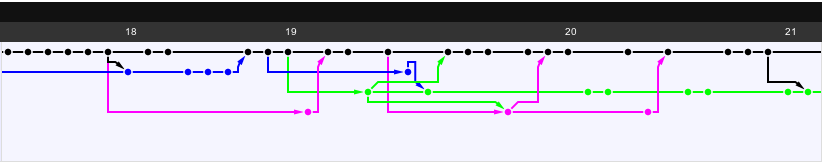
\includegraphics[height=1.3cm,width=7cm]{line2}\\
  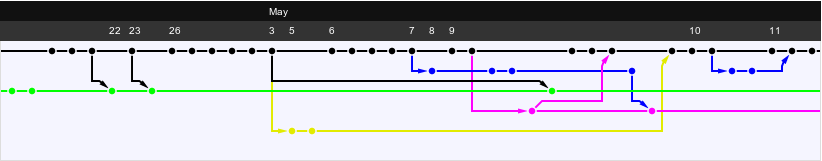
\includegraphics[height=1.3cm,width=7cm]{line3}\\
  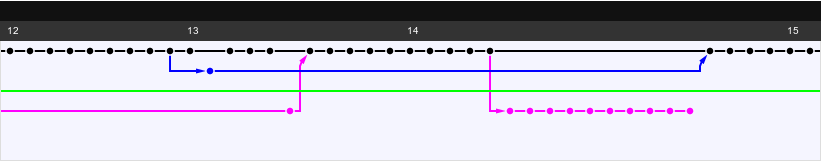
\includegraphics[height=1.3cm,width=7cm]{line4}\\
  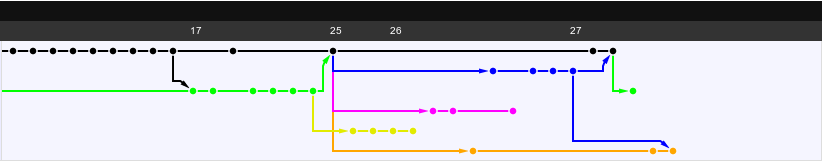
\includegraphics[height=1.3cm,width=7cm]{line5}
  \ecen
\end{frame}


\end{document}
